% Build from this directory with latexmk -pdf report.tex.
\documentclass[11pt,letterpaper]{article}

\usepackage[T1]{fontenc}
\usepackage{newtxtext,newtxmath}
\usepackage[margin=0.78in,bottom=0.72in]{geometry}
\usepackage{graphicx}
\usepackage{booktabs,tabularx}
\usepackage{caption}
\usepackage{float,titlesec}
\usepackage[authoryear,square]{natbib}
\usepackage[colorlinks=true,citecolor=blue,linkcolor=blue,urlcolor=blue]{hyperref}

\linespread{0.94}
\raggedbottom
\titlespacing*{\section}{0pt}{13pt}{6pt}
\titlespacing*{\subsection}{0pt}{8pt}{4pt}
\setlength{\intextsep}{8pt plus 2pt minus 2pt}
\setlength{\parindent}{0pt}
\setlength{\parskip}{4pt plus 1pt minus 1pt}
\setlength{\bibsep}{3pt}
\setcounter{secnumdepth}{1}
\captionsetup{font=small,skip=5pt,labelsep=period,justification=justified,singlelinecheck=false}
\newcolumntype{Y}{>{\centering\arraybackslash}X}
\newcolumntype{L}[1]{>{\raggedright\arraybackslash}p{#1}}

\ifdefined\pdfinterwordspaceon
  \pdfinterwordspaceon
\fi

\begin{document}

\begin{center}
{\Large\bfseries Learning to Select CUDA Thread Block Sizes\\From Kernel Code and Workload Dimensions\par}
\vspace{4pt}
[Author names]\\
New York University, [course and term]\\
{\small\texttt{[NYU email addresses]}}
\end{center}

\begin{abstract}
Choosing a CUDA thread-block size affects kernel runtime, and benchmarking every candidate incurs a tuning
cost. Starting from the published LS-CAT predictor, we ask how much LLVM IR information a launch selector
needs to retain. Our model learns gates over LSTM states, caches the surviving states at build time, and
uses workload dimensions to score candidate sizes at runtime. A 12-kernel pilot collapsed to one retained
state by epoch 10. On 2,785 held-out LS-CAT cases, adaptive retention pruned 16.7\% of optional gates and
achieved 5.54\% mean runtime regret at its selected epoch, compared with 5.48\% for the full-sequence model.
Across 13 live cases, toolcall achieved 1.05--1.50\ensuremath{\times} speedup over fixed 256-thread blocks
with selection time included.
\end{abstract}

\section{Introduction}

A CUDA launch divides work into a grid of thread blocks. A GPU schedules blocks onto streaming
multiprocessors (SMs), where threads execute in warps of 32. For a one-thread-per-item kernel processing
1,000 elements, a 256-thread block requires four blocks and an index check in the last one. A 64-thread
block requires 16 blocks and the same kind of check. Both launches cover the same elements, but they change
the number of blocks the GPU can distribute and the resources allocated to each block.

The useful configuration depends on how the kernel performs its work. More resident warps can help hide
latency. Registers and shared memory can limit residency, and the block shape can affect data reuse, memory
access patterns, and the amount of inactive work near input boundaries. A sweep measures the net effect for
a specific workload, but a production launch may have only one chance to make the decision.

We study a selector that chooses among 16 thread counts from 64 through 1024 in steps of 64. The application
determines the grid that covers its work. Throughout the report, the fastest measured candidate means the
valid tested configuration with the lowest measured time for a specified kernel, input, device, and timing
protocol.

The LS-CAT dataset and its companion predictor showed that LLVM IR contains information about efficient
launch choices \citep{bjertnes2021a,bjertnes2021b}. We started with that separation of code and
workload inputs and examined where to reduce the cost of a prediction. An LSTM can summarize the entire
kernel in its final state, but that single vector may hide details available at intermediate positions.
Keeping every state exposes those details and requires scoring work proportional to the number of states. We
test whether the model can learn a smaller, kernel-specific representation that still chooses a fast
configuration.

We follow this question from the 12-kernel pilot to a larger source-group-held-out LS-CAT experiment and
then to a CUDA launch that includes measured CPU selection time. The deployment test matters because even a
good block prediction only saves time when the faster GPU launch repays the cost of making it.

\section{Literature Survey}

\subsection{Architecture guided and static tuning}

Architecture-guided tuning explains performance using the resources a kernel consumes. Dense linear algebra
experiments showed that register blocking and instruction-level parallelism can yield high performance at
lower occupancy \citep{volkov2008}. This gives a reason to treat occupancy as one factor in launch
selection. A static CUDA autotuner combines program analysis and GPU characteristics to select parameters
without running each configuration \citep{lim2017}. Static approaches avoid per-case measurement when their
models capture the relevant bottlenecks. The assumptions in those models determine how well the
recommendations transfer.

\subsection{Measurement based autotuning}

Empirical autotuners run candidate implementations and search for the fastest measured configuration. Kernel
Tuner \citep{vanwerkhoven2019} searches parameterized GPU kernels and can tune block dimensions jointly with
choices such as tiling or unrolling. Measuring on the target workload captures interactions that a simple
analytic model can miss. The evaluation cost grows as the candidate space expands, and a new input or device
can require another search. In this project, sweeps serve as training data and reference measurements. The
deployed selector makes its decision with one model evaluation.

\subsection{Learning from program representations}

Learned tuning replaces some search with predictions from previous measurements. A study of OpenCL stencils
compared classifiers and performance regressors for workgroup-size prediction \citep{cummins2016}. The
comparison illustrates why runtime loss matters when several configurations have similar performance. LS-CAT
supplies measured runtimes for CUDA kernels collected from public repositories \citep{bjertnes2021a}. A
follow-up study used LLVM IR token sequences and learned embeddings to predict launch choices from this
corpus \citep{bjertnes2021b}. The approach can make a prediction for an unmeasured workload, and its
reliability depends on representative training data and separation of related source code during evaluation.

The LS-CAT prediction study motivates the code encoder in this project. We extend that design by comparing a
workload-only model with full and selectively retained code representations, then embedding a trained
selector in a CUDA host program. This lets us ask whether the code representation earns its runtime cost, a
question that an offline score alone cannot answer.

\section{Proposed Idea}

\subsection{From the published predictor to adaptive retention}

In the original LS-CAT predictor, device LLVM IR passes through a frozen FastText representation and an
LSTM. The authors also evaluated an LSTM encoder--decoder with self-attention. The recurrent output is
transformed and combined with an embedding of the matrix ID. Dense layers then predict a value for each
block size \citep{bjertnes2021b}. We retained the use of IR, a recurrent encoder, separate workload
information, and a vector of candidate predictions. We changed how and when the recurrent output is reduced
so that the scorer can use several informative states and amortize code processing across launches.

\begin{figure}[H]
\centering
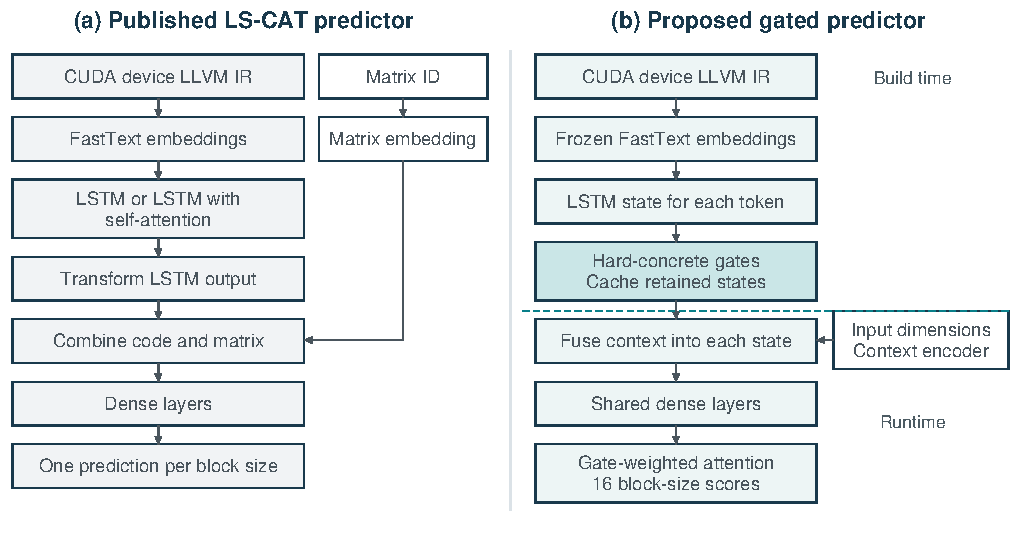
\includegraphics[width=.84\linewidth]{figures/architectures.pdf}
\caption{The published LS-CAT predictor, redrawn from Figure 1 of \citep{bjertnes2021b}, and the proposed gated
predictor. The dashed line marks the handoff from the cached code representation to runtime scoring.}
\label{fig:architectures}
\end{figure}

\subsection{Candidate measurements and training targets}

For each kernel and input shape, the training table contains runtimes for all 16 thread counts. The LS-CAT
import maps a physical block of shape (1, B) to the candidate thread count B. Deployment kernels can realize
that count with a different block shape if their indexing requires it. Keeping the candidate catalog small
makes it practical to record a complete runtime vector and train a scorer that considers the relative cost
of every choice.

If \(T(B)\) is the measured runtime for a candidate and \(T^*\) is the fastest candidate runtime, the target
for B is \(\bigl(T^*/T(B)\bigr)^{12}\). The target reaches one at the measured minimum and falls as runtime
increases. Binary cross-entropy trains the 16 logits against these soft targets, so a close runner-up
receives a stronger target than a slow block. The project's runtime-ratio formula uses the exponent
motivated by the earlier LS-CAT study \citep{bjertnes2021b}.

\subsection{Kernel representation from LLVM IR}

Clang emits LLVM IR for the CUDA device code. The frontend tokenizes the IR and maps tokens to frozen
40-dimensional FastText vectors \citep{bojanowski2017}. An LSTM \citep{hochreiter1997} reads every embedded
token in order and produces one state per token. The gate for a position reads that position's state
together with the final LSTM state. This pairing lets a gate compare a local summary with a summary of the
full kernel. The final state is always retained, so even the most compressed representation contains a state
that has read the full input.

The optional gates use the hard-concrete construction \citep{louizos2018}. Training samples continuous gate
values with a probability of exactly zero and adds a penalty proportional to the expected number of open
states. Evaluation uses deterministic gate values. It removes zero-gated rows and caches the surviving
hidden states and gate values. Gate selection depends on the kernel code, so the representation can be
reused across input dimensions. Every token is still encoded at build time. Closing gates saves storage and
reduces the number of rows scored at runtime.

\subsection{Dense layers and attention}

The workload encoder log-scales the dimensions and projects them into 32 features. We concatenate that
context with every retained state and run the same dense layers on each row, with hidden sizes of 256, 128,
and 64. Each row produces 16 block-size logits and a scalar attention score. The model multiplies the
attention weights by the gate values and renormalizes across the retained rows. The weighted sum yields one
logit per block size. Workload-dependent attention can emphasize different parts of the same cached
representation at different input sizes.

The context-only control scores the dimensions alone. The final-state comparison keeps one complete-input
summary, and the full-sequence model scores every state. The adaptive model learns its own retention count.
These comparisons test whether intermediate states carry useful information and whether the model can
discard part of the sequence while preserving the quality of its block choices.

\subsection{Compiling and launching a user kernel}

To use the selector, include \texttt{toolcall.hpp} in the CUDA host code and call \texttt{model\_output}
with the kernel and workload. The API returns the grid and block dimensions for one-dimensional coverage.
The scorer masks unsupported candidates using device and kernel launch limits. The wrapper accepts explicit
\texttt{work\_items} so launch coverage follows the indexing of the kernel, while m, n, and k provide the
model's workload features.

\begin{verbatim}
#include "toolcall.hpp"
auto [grid, block] = toolcall::model_output(my_kernel, {m, n, k, work_items});
my_kernel<<<grid, block>>>(device_args);
\end{verbatim}

Build the executable with \texttt{./toolcall my\_kernel.cu -o my\_program}. The wrapper extracts the
kernel's LLVM IR, runs the encoder and gates, and includes the cached representation in the launch
artifacts. Softmax uses one thread per vector, so its grid rounds up the vector count. ComputeOrientations
assigns a warp to each keypoint. Matrix multiply + ReLU uses 32 columns per block tile and derives the tile
height and grid from the predicted thread count.

\subsection{Native and compiled CPU scorers}

The native path implements the context encoder, dense layers, and attention directly in C++ with weights
generated from the checkpoint. With \texttt{--aot}, PyTorch's AOTInductor exports and compiles the same CPU
scoring graph and packages its trained weights. The CUDA host program loads the compiled package through
LibTorch. Both backends use the same \texttt{model\_output} API and run the user's kernel on the GPU. The
compiled path specializes the scoring graph for the cached state count, which is known when the program is
built.

\section{Experimental Setup}

\begin{table}[H]
\centering\small
\caption{Devices and software used for the recorded experiments.}
\begin{tabularx}{\linewidth}{@{}L{.19\linewidth}L{.32\linewidth}>{\raggedright\arraybackslash}X@{}}
\toprule
\textbf{Experiment} & \textbf{Device} & \textbf{Recorded software or source} \\
\midrule
Local 1D sweeps & RTX 2080 Ti \textbullet{} 68 SMs \textbullet{} CC 7.5\newline A100-SXM4-40GB \textbullet{} 108 SMs \textbullet{} CC 8.0 & Linux and NVCC 13.0.88. Device and environment logs are stored with each run. \\
LS-CAT model comparison & NVIDIA T4 for archived labels\newline NVIDIA TITAN V in model timing logs & PyTorch 2.8.0+cu128 and CUDA 12.8 in the model logs. Clang/LLVM and FastText for the frontend. \\
Live launch benchmarks & CPU scorer and CUDA GPU execution & C++17/CUDA benchmark sources and toolcall build wrapper. \\
\bottomrule
\end{tabularx}
\end{table}

\subsection{Local CUDA measurements}

Each one-dimensional run covers 12 kernels and 32 workload contexts, with 16 blocks and 10 repetitions per
context (5,120 valid timings on each GPU). Benchmarks include data movement, reductions, statistics,
softmax, and N-body. The sweep times a single warmed launch with CUDA events. Small outputs receive full CPU
reference checks. Larger outputs receive 64 deterministic reference checks, a scan for invalid output, and
guard checks. Use each run's source snapshot, \texttt{metadata.json}, \texttt{contexts.json}, and
\texttt{heavy\_action\_table.csv} to recover its inputs, seeds, launch geometry, and median timings. The
hardware comparison joins on kernel and all three dimensions. The runs use different generated seeds. The
initial retention pilot used the RTX 2080 Ti collection and trained on 27 contexts from ten kernels.
Validation used five contexts from two held-out kernels. We logged retention for each epoch to detect
collapse to the mandatory final state.

% Draft note: Local collections under data/ are one-d-full-20261112T042718Z-Smx6nn-cuda2 and one-d-
% full-20261112T050931Z-xcKanr-hpc-a100. The recorded input and launch details are in each collection’s
% contexts.json, metadata.json, and heavy_action_table.csv.

\subsection{Model validation on the public CUDA corpus}

Following the pilot, we imported the full available one-dimensional set from the public LS-CAT T4 archive.
The import script, \texttt{scripts/import\_lscat.py}, keeps complete 16-candidate cases, averages duplicate
archived timings, and drops invalid timings. The frontend and FastText scripts prepare token IDs and
matching frozen embeddings. The saved split contains 400 source groups for training (2,050 kernels, 16,423
cases) and 50 groups for validation (338 kernels, 2,785 cases). The same source group stays on one side of
the split.

% Draft note: Confirm the exact LS-CAT archive revision, device IR generation command and target, Clang
% version, and the corpus used to fit the vocabulary and embeddings. Record the original training artifact
% paths and file hashes.

Recreate the saved comparison with \texttt{scripts/train\_adaptive.py} and the split stored in the
checkpoint. Use model and split seed 2, 120 epochs, batch size 8, AdamW at 0.001, zero weight decay,
gradient clipping at 1, and BCE targets with exponent 12. The sequence models use LSTM width 1. The adaptive
runs use a length penalty of \(10^{-8}\) with KL weights of 0 and \(10^{-4}\). For the KL run, the
temperature is 2 and the teacher decay is 0.99. Checkpoints are selected by validation regret, then task
loss.

\subsection{Live timing protocol}

Build the fixed and toolcall variants from \texttt{examples/runtime\_launch} and pass the inputs and block
sizes recorded in the CSV for each sweep. Use \texttt{scripts/collect\_launch\_benchmarks.py} to collect
results. After five warm-ups, the benchmark records medians over 51 trials for CPU selection time, GPU time,
and host time from selection to synchronized kernel completion. The GPU event timer uses a separate launch.
The reported host interval begins after buffer setup and ends before output verification.

% Draft note: Confirm the CPU, GPU, driver, compiler versions and flags, checkpoint, scorer backend, and CPU
% thread settings for each archived sweep. The wrapper defaults to sm_75 and
% lscat_adaptive_h1_lambda1e-8_no-kl_ep120.best.pt. The reference CSVs are
% softmax_20261121T135731_523919.csv, matrix_multiply_and_relu_20261121T221009_455918.csv,
% compute_orientations_20261121T164854_894079.csv in results/launch_benchmarks.

The softmax sweeps use 150,051 or 180,051 vectors of length 1,500 and 150,051 or 200,051 vectors of length
2,000. The ReLU sweep uses square matrices of side 5,632, 6,144, 6,656, or 7,168. Orientation uses a
4,096-pixel-square image with keypoint counts from 56,194,304 to 72,194,304 in increments of 4,000,000. The
softmax and ReLU fixed sweeps add candidates near the selected size to the 16-count catalog. Orientation
sweeps 32, 64, 128, 256, 384, 512, and 576.

\section{Experiments \& Analysis}

\subsection{Measures of success}

For each validation case, regret is 100 \ensuremath{\times} (selected runtime / fastest measured runtime
\ensuremath{-} 1). The performance score is the mean of fastest measured runtime divided by selected
runtime. Exact-winner rate counts predictions of the measured minimum. For deployment, speedup is the
fixed-run median host time divided by the model-run median host time. A value above one means the GPU time
saved was sufficient to cover selection for the recorded workload. Retained-state fraction measures how much
of the original sequence the scorer must process.

\subsection{Block size sensitivity}

\begin{figure}[H]
\centering
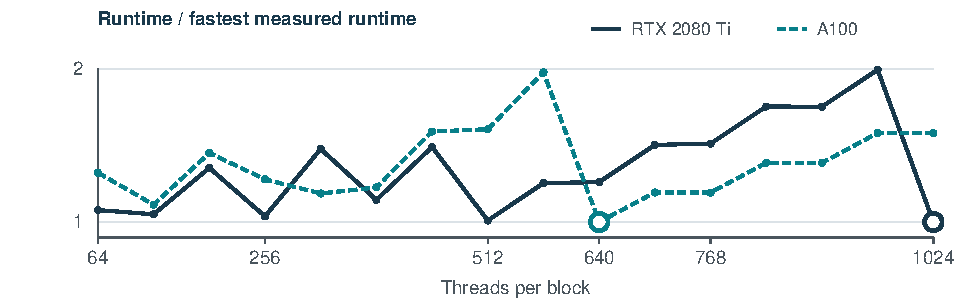
\includegraphics[width=.92\linewidth]{figures/nbody.pdf}
\caption{N-body with 65,536 bodies. Runtimes are normalized to the fastest measured candidate on each GPU. Rings mark
the measured minima.}
\label{fig:nbody}
\end{figure}

The 640-thread block ran in 7.54 ms on the A100, versus 11.91 ms at 1024 threads. On the RTX 2080 Ti, the
same 640-thread choice took 11.03 ms, versus 8.76 ms at 1024. Across the 24 matching kernel-and-shape pairs,
measured winners agreed in 11. Some rankings change within a nearly flat region of the runtime curve. In the
N-body example, the gaps span several milliseconds, while the median absolute deviations for these four
timings were below 0.05 ms. Device resources and kernel tiling can both influence the curves.

\subsection{Gate collapse in the 12 kernel pilot}

The early adaptive model started with a mean of 1,563.6 retained states per validation case. In the
width-eight run, the mean dropped to 8.8 states at epoch 8 and reached one at epoch 9. By epoch 10, all five
validation cases retained only the final state. This reduction was an early sign that the small training set
offered too little evidence to learn which intermediate states mattered across kernels. The length penalty
also rewarded early pruning. We expanded the dataset to improve coverage and used a smaller length penalty
in the later runs.

\begin{figure}[H]
\centering
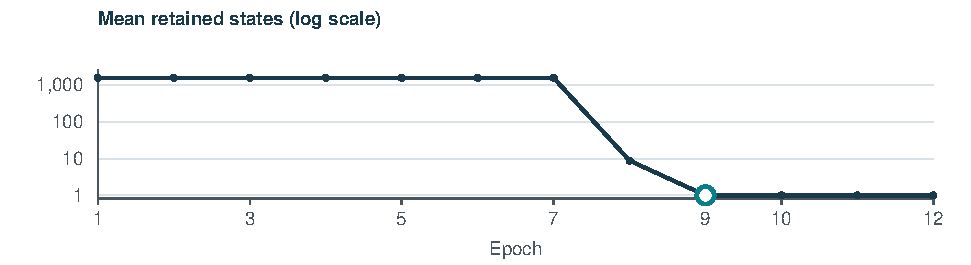
\includegraphics[width=.92\linewidth]{figures/pilot_retention.pdf}
\caption{Mean validation retention during the first 12 epochs of the width-eight pilot. The vertical axis is
logarithmic. The ring marks the first epoch with one state per validation case.}
\label{fig:pilot_retention}
\end{figure}

\subsection{Validation regret and retained states}

\begin{table}[H]
\centering\small
\caption{LS-CAT results at each model's best-validation-regret epoch.}
\begin{tabularx}{\linewidth}{@{}L{.24\linewidth}YYYYY@{}}
\toprule
\textbf{Model} & \textbf{Epoch} & \textbf{Mean regret} & \textbf{Performance score} & \textbf{Exact winner} & \textbf{Optional states kept} \\
\midrule
Context only & 78 & 5.65\% & 0.9508 & 9.30\% & --- \\
Full sequence & 50 & 5.48\% & 0.9519 & 8.65\% & 100.0\% \\
Adaptive without KL & 41 & 5.54\% & 0.9517 & 8.62\% & 83.3\% \\
Adaptive with KL & 31 & 5.59\% & 0.9512 & 7.90\% & 100.0\% \\
\bottomrule
\end{tabularx}
\end{table}

Full retention achieved the lowest mean regret on the validation split. Without KL, learned retention pruned
16.7\% of optional states at its selected epoch and was within 0.06 percentage points of full retention in
mean regret. Its exact-winner rate was 8.62\%, close to 8.65\% for all states. The near match suggests that
many states can be removed while preserving the information needed for good block choices on this split.
Exact winners remain uncommon because the metric requires the single measured fastest block even when
several choices cost almost the same time.

\begin{table}[H]
\centering\small
\caption{Final-state intervention at epoch 120. Each pair uses the same trained adaptive checkpoint and workload cases.}
\begin{tabularx}{\linewidth}{@{}L{.22\linewidth}YYYY@{}}
\toprule
\textbf{Training run} & \textbf{Exact winner with learned retention} & \textbf{Exact winner with final state} & \textbf{Mean regret with learned retention} & \textbf{Mean regret with final state} \\
\midrule
Adaptive without KL & 8.94\% & 7.07\% & 9.90\% & 9.27\% \\
Adaptive with KL & 8.65\% & 6.86\% & 7.48\% & 19.91\% \\
\bottomrule
\end{tabularx}
\end{table}

We forced the scorer to use one state by passing only the mandatory final state to an already-trained model.
Exact-winner accuracy fell for both checkpoints, showing that the intermediate states carry information used
by the scorer. Mean regret increased for the KL checkpoint and improved slightly for the no-KL checkpoint.
Exact-winner accuracy measures how often the model is first, while regret reflects how costly its misses
are. The intervention measures the effect of removing states from the same checkpoint at epoch 120.

\subsection{Effect of KL regularization}

We use Kullback--Leibler (KL) divergence to encourage the current model to match the candidate score
distribution of a teacher formed by an exponential moving average of earlier weights. The intent is to
stabilize predictions as the gates change. At their selected epochs, the no-KL run had slightly lower regret
(5.54\% versus 5.59\%) and pruned more optional states (16.7\% versus 0\%). One explanation is that matching
an earlier distribution makes it harder for the scorer and gates to adjust together as states close. The
saved runs support the trade-off at the selected checkpoints. Establishing that mechanism would require
repeated matched runs.

At epoch 120 the no-KL run pruned 38.8\% of optional states, and regret rose to 9.90\%. The KL run pruned
4.5\% and recorded 7.48\% regret at that epoch. This illustrates why the best checkpoint for deployment may
differ from the one with the smallest representation. A small loss in block selection quality can be
worthwhile if processing fewer rows saves more CPU time than the selected block loses on the GPU. We measure
the two costs together at launch.

\subsection{Live launch performance}

\begin{table}[H]
\centering\small
\caption{Deployment results using host time from selection through completion.}
\begin{tabularx}{\linewidth}{@{}L{.24\linewidth}YYYYY@{}}
\toprule
\textbf{Benchmark} & \textbf{Cases} & \textbf{Model threads} & \textbf{Best fixed threads} & \textbf{Speedup vs. 256} & \textbf{Gap to best fixed} \\
\midrule
Softmax & 4 & 576 & 544/576 & 1.41--1.50\ensuremath{\times} & 0.49--9.36\% \\
Matrix multiply + ReLU & 4 & 512 & 1024 & 1.20--1.21\ensuremath{\times} & 0.70--1.01\% \\
ComputeOrientations & 5 & 64 & 64 & \ensuremath{\approx}1.055\ensuremath{\times} & 0.16--0.33\% \\
\bottomrule
\end{tabularx}
\end{table}

\begin{figure}[H]
\centering
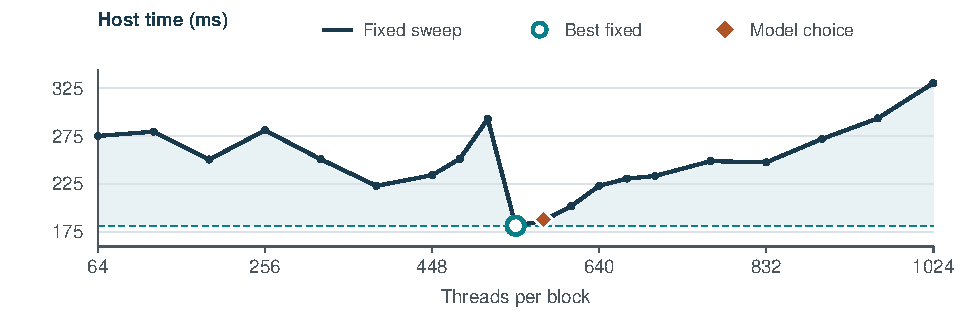
\includegraphics[width=.92\linewidth]{figures/softmax.pdf}
\caption{Softmax with 150,051 vectors of length 1,500. The shaded area shows excess time above the fastest observed
fixed launch. The model selected 576 threads, and the fastest fixed candidate used 544.}
\label{fig:softmax}
\end{figure}

For the softmax input in Figure~\ref{fig:softmax}, the model took 187.85 ms compared with 281.19 ms at fixed
256 and 181.52 ms at fixed 544. At fixed 576, the same block chosen by the model took 186.68 ms. The
same-block comparison shows a 1.17 ms difference in total time, close to the separately recorded 1.16 ms
selection time. The 256-thread block had enough headroom for the prediction to pay off. The 544-thread fixed
candidate kept a smaller advantage over the model.

For matrix multiply + ReLU, the model's 512-thread choice was near the best measured fixed 1024-thread
launch. A 512-thread block covers 16 rows per tile and a 1024-thread block covers 32. Changing rows per tile
changes the work per block and shared memory usage. For ComputeOrientations, the model chose the same block
size as the best fixed run on every input. Each warp has its own scratch space, so larger blocks request
more shared memory. Profiling would be needed to distinguish residency, reuse, and scheduling effects. The
model saved time against fixed 256 in both workloads.

The deployed checkpoint retained 3,165 of 3,165 states on softmax, 1,301 of 3,566 on matrix multiply + ReLU,
and 2,076 of 11,149 on ComputeOrientations. Measured selection medians across the three kernels ranged from
1.06 to 1.46 ms. The cases differ in code, input, and kernel duration. A matched run using alternate
retention counts for the same kernel would be needed to measure the effect of pruning on selection time.

\subsection{Scorer backend comparison}

In the development tests, the team observed substantially faster CPU scoring with the AOTInductor package
than with the native C++ implementation. A plausible contributor is that AOTInductor compiles the scoring
graph into optimized CPU code specialized for the cached state dimensions. The archived launch sweeps lack
matched native and AOT rows with recorded backend and build settings, so we report the direction observed in
development and leave its speedup unquantified.

% Draft note: Add paired native and AOT median selection and total times when available. Use the same
% kernel, shape, checkpoint, retention count, CPU thread settings, and warm-up for both backends. The first
% AOT invocation loads the package.

\subsection{When to use the selector}

The break-even test is whether the GPU time saved over the current fixed block exceeds the extra CPU
selection time. Large workloads are good candidates when the difference between the baseline block and a
fast block grows in absolute time. In the softmax example, total time fell by 93.34 ms against fixed 256,
while a same-block comparison put the added cost at about 1.17 ms. The available gain is specific to the
workload and reference block.

For the block-size versus runtime plots, the excess area above the measured minimum describes how sensitive
the sweep is to block choice. A small area after normalizing for the minimum runtime means many blocks are
close to the best in relative terms. It makes a slightly imperfect prediction less costly, while also
leaving less tuning headroom when the fixed baseline lies in the same flat region. Even a small relative
difference on a long-running kernel can exceed the selection cost in milliseconds. The gap from the actual
fixed baseline to the selected block is the quantity to compare with that cost.

\subsection{Scope of the results}

The live sweeps use long-running kernels and report within-run medians. The ReLU and orientation examples
draw on source kernels in the LS-CAT validation partition. These experiments establish deployment behavior
for the recorded cases. An independent test set, repeated measurement sessions, and verified training-only
frontend fitting would strengthen claims about generalization and small timing differences.

% Draft note: The three tables and plots use the recorded one-dimensional, LS-CAT, and runtime evidence. The
% sigmoid sweep is excluded because the same-block GPU times differ substantially between binaries. Verify
% its build and run conditions before incorporating it.

\section{Conclusions}

\begin{itemize}

\item Measured block-size sensitivity varied with the kernel, workload, and GPU. On the 65,536-body case, the
fastest tested block was 1024 threads on the RTX 2080 Ti and 640 on the A100.

\item The 12-kernel pilot collapsed to one state. On the larger LS-CAT split, the selected no-KL checkpoint pruned
16.7\% of optional states and reached 5.54\% mean regret, close to the full sequence's 5.48\%.

\item Toolcall improved total time over fixed 256 across all 13 recorded cases, including CPU selection. The
fastest swept fixed configuration retained an advantage in each case. The selector pays off when savings
over the existing block exceed prediction overhead.

\end{itemize}

\begin{thebibliography}{9}
\small

\bibitem[Bjertnes et al.(2021a)]{bjertnes2021a}
Lars Bjertnes, Jacob O. Tørring, and Anne C. Elster, ``LS-CAT: A Large-Scale CUDA AutoTuning Dataset,'' in
IEEE International Conference on Applied Artificial Intelligence (ICAPAI), 2021a.

\bibitem[Bjertnes et al.(2021b)]{bjertnes2021b}
Lars Bjertnes, Jacob O. Tørring, and Anne C. Elster, ``Autotuning CUDA: Applying NLP Techniques to LS-CAT,''
in Norsk informatikkonferanse (NIKT), pp. 72--85, 2021b.

\bibitem[Bojanowski et al.(2017)]{bojanowski2017}
Piotr Bojanowski, Edouard Grave, Armand Joulin, and Tomas Mikolov, ``Enriching Word Vectors with Subword
Information,'' Transactions of the Association for Computational Linguistics, vol. 5, pp. 135--146, 2017.

\bibitem[Cummins et al.(2016)]{cummins2016}
Chris Cummins, Pavlos Petoumenos, Michel Steuwer, and Hugh Leather, ``Autotuning OpenCL Workgroup Size for
Stencil Patterns,'' in 6th International Workshop on Adaptive Self-Tuning Computing Systems, 2016.

\bibitem[Hochreiter and Schmidhuber(1997)]{hochreiter1997}
Sepp Hochreiter and Jürgen Schmidhuber, ``Long Short-Term Memory,'' Neural Computation, vol. 9, no. 8, pp.
1735--1780, 1997.

\bibitem[Lim et al.(2017)]{lim2017}
Robert V. Lim, Boyana Norris, and Allen D. Malony, ``Autotuning GPU Kernels via Static and Predictive
Analysis,'' in 46th International Conference on Parallel Processing (ICPP), pp. 523--532, 2017.

\bibitem[Louizos et al.(2018)]{louizos2018}
Christos Louizos, Max Welling, and Diederik P. Kingma, ``Learning Sparse Neural Networks through \(L_0\)
Regularization,'' in 6th International Conference on Learning Representations (ICLR), 2018.

\bibitem[van Werkhoven(2019)]{vanwerkhoven2019}
Ben van Werkhoven, ``Kernel Tuner: A Search-Optimizing GPU Code Auto-Tuner,'' Future Generation Computer
Systems, vol. 90, pp. 347--358, 2019.

\bibitem[Volkov and Demmel(2008)]{volkov2008}
Vasily Volkov and James W. Demmel, ``Benchmarking GPUs to Tune Dense Linear Algebra,'' in Proceedings of the
ACM/IEEE Conference on Supercomputing (SC), 2008.

\end{thebibliography}

\end{document}
